Our test were performed mainly on two machines: one with an Intel® Core i7-7700 @ $3.6 \ GHz$ with $16 \ GB$ of RAM and one on an AMD® Ryzen 7 @ $3.6 \ GHz$ with $32 \ GB$ of RAM.
\subsection{Monte Carlo PERM}
We want now to report an application of the PERM algorithm, made following the article's recipe \cite{PERM}.
The goal of this algorithm is to estimate the total number of fold and then simulate a finite number of SRCs hoping to find the energy minimum.
In the article the number of iterations is set to be $10^5$ for all proteins and the result is that they found only local minima, which are intermediate states.
Our goal is to improve these 2D simulations by increasing the number of iterations, hoping to find the real minimum reported in a famous benchmark \cite{bench}.

The first protein for which we've improved the result is $HH(P)^5HH(P)^3H(P)^3HP$, that has a length of 18 amino acids (see Fig. \ref{fig:18_1}).
In particular, we've found $(1.25 \pm 0.35) \times 10^8$ folds with an energy minimum of -4 (a.u.), equal to the benchmark's one.
\begin{figure}[H]
    \centering
    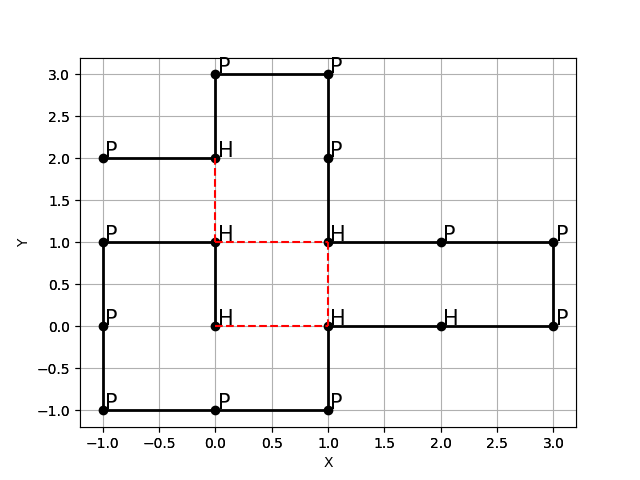
\includegraphics[width=.75\textwidth]{./img/18_1.png}
    \caption{\emph{The protein $HH(P)^5HH(P)^3H(P)^3HP$ has reached its energy minimum at -4 (a.u.) after $5 \times 10^6$ iterations ($\sim 20$ minutes).}}
    \label{fig:18_1}
\end{figure}
Another protein for which we've improved the result is $HHHP(PH)^3PP(HP)^3PH$, that has a length of 20 amino acids (see Fig. \ref{fig:20_2}).
In this case, we've found $(8.9688 \pm 0.0033) \times 10^{10}$ folds with an energy minimum of -9 (a.u.), one unit more than the benchmark's one.
\begin{figure}[H]
    \centering
    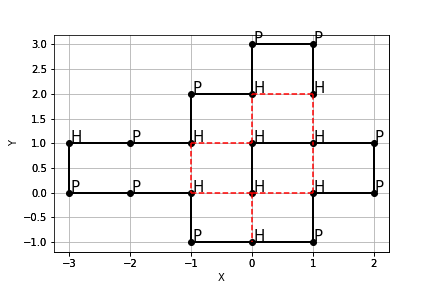
\includegraphics[width=.75\textwidth]{./img/20_2.png}
    \caption{\emph{The protein $HHHP(PH)^3PP(HP)^3PH$ has reached an energy minimum of -9 (a.u.) after $10^7$ iterations ($\sim 45$ minutes).}}
    \label{fig:20_2}
\end{figure}
We've also tried to improve the protein $HPHPHHH(P)^3HHHH(P)^2HH$, that has a length of 20 amino acids (see Fig. \ref{fig:18_2}).
However, after about 5 hours of running time it has folded with an energy of -7 (a.u.), like in the article, with an estimated number of folds equal to $(1.24 \pm 0.43) \times 10^8$.
\begin{figure}[H]
    \centering
    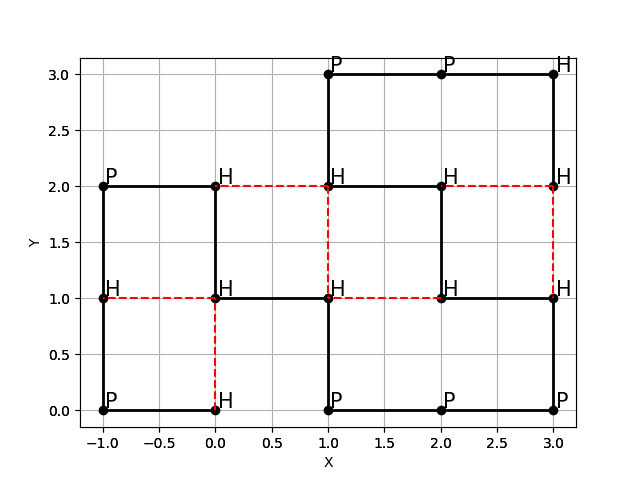
\includegraphics[width=.75\textwidth]{./img/18_2.png}
    \caption{\emph{The protein $HPHPHHH(P)^3HHHH(P)^2HH$ has reached an energy minimum of -7 (a.u.) after $10^8$ iterations ($\sim 5$ hours).}}
    \label{fig:18_2}
\end{figure}

\subsection{Constraint-based Protein Structure Prediction PERM}
In the 2D case we showed that increasing the number of iterations resulted in better estimate of the energy.
However, the previous algorithm is not able to give significant outputs in the 3D case.
We tried so to estimate the energy in the 3D case with another algorithm, which is also based on constraint programming.
This is implemented by \emph{CPSP-tools} \cite{cpsp} and has revealed to be very powerful, folding proteins of length $\sim 200$ in few seconds.
Furthermore, this program is able to fold proteins in more complex lattices, like the 3D-face-centered-cubic one.
In our case, we wanted to improve the results of article \cite{PERM} so, in order to keep consistency, we opted for a 3D-cubic lattice.
All proteins tested converged to their minima, as we can see in Fig. \ref{fig:cpsp}.

\begin{figure}[H]
    \centering
    \begin{subfigure}[b]{0.45\textwidth}
        \centering
        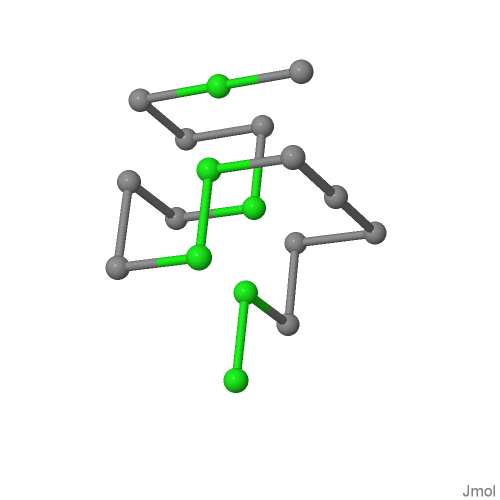
\includegraphics[width=\textwidth]{./img/18_3D.png}
        \caption{\emph{Energy $-4$ (a.u.) for the sequence $HH(P)^5HH(P)^3H(P)^3HP$.}}
    \end{subfigure}
    \begin{subfigure}[b]{0.45\textwidth}
        \centering
        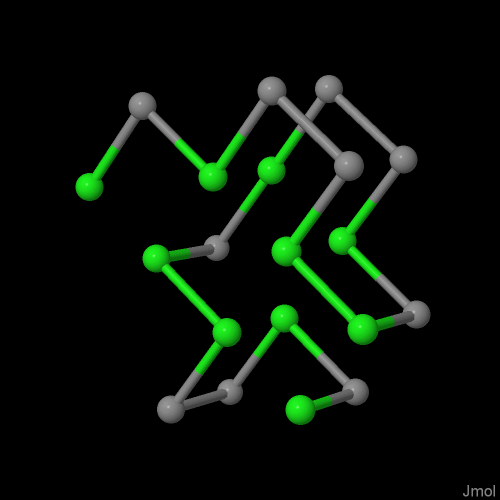
\includegraphics[width=\textwidth]{./img/20_3D.png}
        \caption{\emph{Energy $-11$ (a.u.) for the sequence $(HP)^2PH(HP)^2(PH)^2HP(PH)^2$.}}
    \end{subfigure}
    \begin{subfigure}[b]{0.45\textwidth}
        \centering
        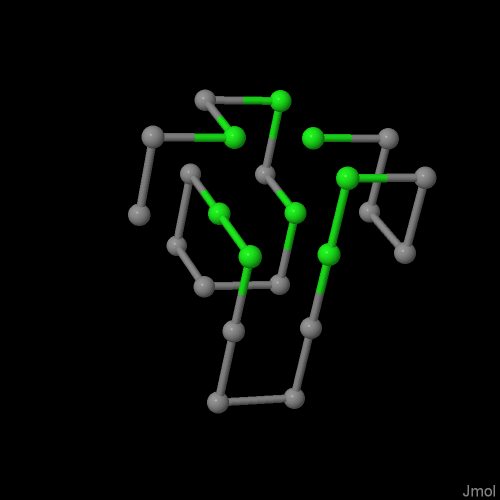
\includegraphics[width=\textwidth]{./img/24_3D.png}
        \caption{\emph{Energy $-8$ (a.u.) for the sequence $P(PH)^3(P)^4(HH(PP)^2)^2H$.}}
    \end{subfigure}
    \begin{subfigure}[b]{0.45\textwidth}
        \centering
        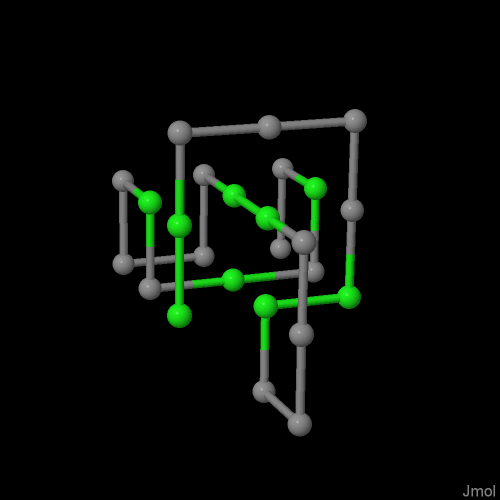
\includegraphics[width=\textwidth]{./img/25_3D.png}
        \caption{\emph{Energy $-8$ (a.u.) for the sequence $P(PH)^3(P)^4(HH(PP)^2)^2HH$.}}
    \end{subfigure}

    \caption{\emph{Four proteins of length 18 (a), 20 (b), 24 (c) and 25 (d).}}
    \label{fig:cpsp}
\end{figure}


\subsection{Reinforcement Learning}

Due to the fact that Reinforcement Learning code is extremely hard to write and optimize performance-wise, this section will only report the main results obtained with DRL algorithms by \cite{jafari2020solving}. These results are enough to show that DRL outperforms PERM and more in general bruteforce methods

\FloatBarrier
\begin{table}[ht!]
\centering
\begin{tabular}[c]{ |p{6cm}||p{3cm}||p{3cm}|}
 \hline
 \multicolumn{3}{|c|}{Performance} \\
 \hline
 Sequence  & PERM & DRL\\
 \hline
(HP)2PH2PHP
2HPH2P2HPH & Less than a second & Less than a second\\
 \hline
P2HP2H2P4H
2P4H2P4H2 & 6 seconds  & Less than a second\\
 \hline
P3H2P2H2P5H7P
2H2P4H2P2HP2 & Less than a second & Less than a second\\
\hline
P2HP2H2P2H2P5H10
P6H2P2H2P2HP2H5 & 3 minutes & 25 seconds\\
\hline
H2(PH)3PH4PHP3
HP3HP4HP3HP3HP
H4(PH)3PH2 & 3 seconds & Less than a second\\
\hline
P2H3PH8P3H10PH

P3H12P4H6PH2PHP & 7 seconds & Less than a second\\
\hline 
H12(PH)2(P2H2)2P2
H(P2H2)2P2HPHPH12 & 78 hours & 48 minutes\\
\hline
H4P4H12P6(H12P3)
3HP2(H2P2)2HPH & 64 seconds & 16 seconds\\
\hline
P3H2P2H4P2H3(PH2)3
H2P8H6P2H6P9HPH2PH11
P2H3PH2PHP2HPH3P6H3 & 1 hour & 4 minutes\\
\hline
P6HPH2P5H3PH5PH2(P2H2)
2PH5PH10PH2PH7P11H7P2

HPH3P6HPHP2 & 9 minutes & 1 minute\\
\hline

\end{tabular}\\
\caption{Performance of Perm and Deep Reinforced Learning on the same protein sequence, the energy was omitted because for each sequence both model found the same energy of the folded state}
\end{table}

\FloatBarrier

